\section{Results}
\label{results_section}

\begin{table}[t]
	\centering
	\footnotesize
	\begin{tabular}{l r r r}
		\toprule
			\bfseries Model & \Pc{} & \Cc{} & \Oc{} \\
		\midrule
			\smallflan{}  & 248 & 4284 & 228 \\
			\bigflan{} & 242 & 4304 & 214 \\
		\midrule
			\smallllama{} & 745 & 3662 & 353 \\
			\bigllama{} & 1070 & 3303 & 387 \\
		\bottomrule \addlinespace[4pt]
	\end{tabular}
	\caption{Amount of answers of each category when running our dataset on each of the four models.}
	\label{total_table}
\end{table}

\begin{figure}[t]
	\centering
	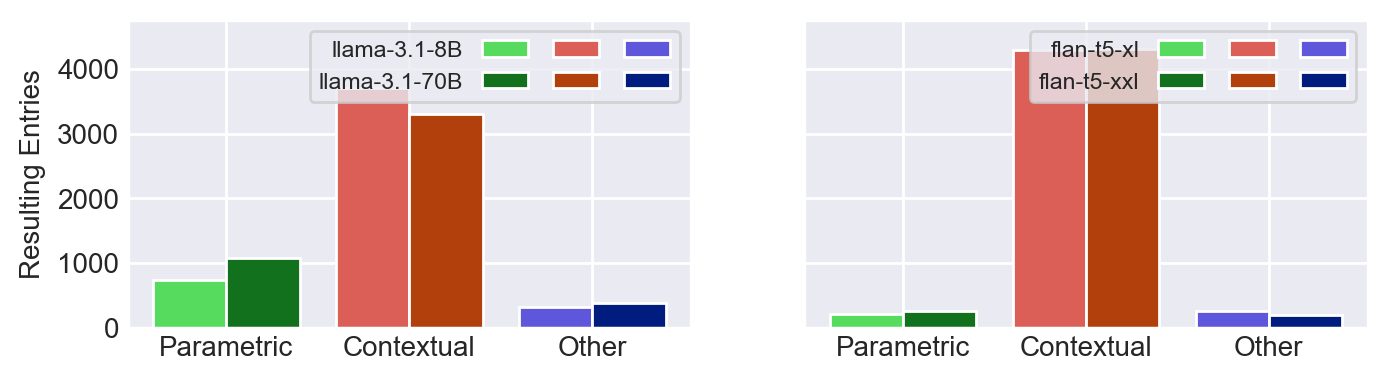
\includegraphics[width=\columnwidth]{both_amount.png}
	\caption{Amount of each answers of each category when running a context with counterparametric information for encoder-decoder and Decoder-only models of different sizes.}
	\label{total_plot}
\end{figure}

\begin{table*}[t]
	\centering
	\footnotesize
	\begin{tabular}{>{\bfseries}l | r r r | r r r | r r r | r r r}
		\toprule
			& \multicolumn{3}{c|}{\smallflan{}} & \multicolumn{3}{c|}{\bigflan{}} & \multicolumn{3}{c|}{\texttt{llama-8B}} & \multicolumn{3}{c}{\texttt{llama-70B}}  \\
			& \Pc{} & \Cc{} & \Oc{} & \Pc{} & \Cc{} & \Oc{} & \Pc{} & \Cc{} & \Oc{} & \Pc{} & \Cc{} & \Oc{}  \\
		\midrule
			Person           &  32 &  900 & 37 &  23 &  890 & 56 &  40 &  833 & 96 & 209 & 614 & 146 \\
			City             & 120 & 1030 & 40 &  78 & 1093 & 19 & 117 & 1007 & 66 & 166 & 966 &  58 \\
			Principle        &  13 &  164 &  8 &   9 &  168 &  8 &  44 &  118 & 23 &  44 & 117 &  24 \\
			Element          &   6 &  637 &  2 & 102 &  515 & 28 & 218 &  385 & 42 & 275 & 347 &  23 \\
			Book             &  26 &  488 & 25 &  18 &  457 & 64 & 135 &  344 & 60 & 154 & 318 &  67 \\
			Painting         &  26 &  446 & 56 &   4 &  498 & 26 &  47 &  458 & 23 &  49 & 445 &  34 \\
			Historical Event &  11 &  217 & 28 &   1 &  254 &  1 &  81 &  154 & 21 & 117 & 118 &  21 \\
			Building         &  14 &  174 & 10 &   0 &  189 &  9 &  27 &  163 &  8 &  31 & 159 &   8 \\
			Composition      &   0 &  228 & 22 &   7 &  240 &  3 &  36 &  200 & 14 &  25 & 219 &   6 \\
		\bottomrule \addlinespace[4pt]
	\end{tabular}
	\caption{Results for each model tested on queries with counterparametric context in each one of the 10 given categories.}
	\label{cats_table}
\end{table*}

The results of running the queries with the questions created in \cref{dataset_creation} with added counterparametric context on each of the four models.

\Cref{total_table} shows the total type of answers for each one of the models.
These numbers represent the amount of answers with a particular source for each one of the models when asking queries for all 4760 questions.

% Of the encoder-decoder models, \smallflan{} has $248$ answers from \Parametric{} knowledge ($5.21\%$), $4284$ answers from \Contextual{} knowledge ($90\%$), and $228$ answers from \Other{} source ($4.79\%$).
% \bigflan{} has a similar distribution of answers with $242$ \Parametric{} answers ($5.08\%$), $4304$ \Contextual{} answers ($90.42\%$), and $214$ \Other{} answers ($4.5\%$).

% The decoder-only models also have a majority of \Contextual{} answers, but have an otherwise different distribution with a smaller majority.
% \smallllama{} has $745$ answers from \Parametic{} knowledge ($15.65\%$), $3662$ answers from \Contextual{} knowledge ($76.93\%$), and $353$ answers from some \Other{} source ($7.42\%$).
% Unlike the previous architecture, the larger model \bigllama{} has a significantly different result with $1070$ \Parametric{} answers ($22.48\%$), $3303$ \Contextual{} answers ($69.39\%$), and $387$ \Other{} answers ($8.13\%$).

This information is plotted in \cref{total_plot}, where the differences between architectures and sizes can be better appreciated.

\Cref{cats_table} contains the information separated by question category.
That is, for each model being tested with counterparametric data added to the context, how many questions in each category have answers from the \Parametric{} knowledge of the model, the \Contextual{} information in the query, and some \Other{} source.

The following sections discuss the reasons for the differences in distributions of the source of these answers along different models, and in the differences between different categories.
